% !TEX root = ../discretemath.tex

\section{Лапласиан графа и теоремы о деревьях}

\subsection{Лапласиан графа}

Рассматриваем \emph{граф $G$ без петель} (с возможными кратными рёбрами).

\begin{Definition}{Лапласиан (матрица Лапласа) графа}{}
	Пусть $G$ — граф на $n$ вершинах. \emph{Лапласиан} $L_G = (l_{ij})_{n\times n}$, где
	\[
	l_{ij} =
	\begin{cases}
		d_i, & i = j,\\
		-(\text{число рёбер между вершинами } i \text{ и } j), & i \neq j,
	\end{cases}
	\]
	и $d_i = \deg i$ — степень вершины $i$.
\end{Definition}

\begin{Remark}{}{}
	Сумма элементов каждой строки (и каждого столбца) лапласиана равна нулю:
	$\displaystyle\sum_{j=1}^{n} l_{ij} = 0$ для всех $i$.
\end{Remark}

\begin{Example}{Лапласиан графа}{}
	Рассмотрим граф $G$ на вершинах $\{1,2,3,4\}$ с рёбрами
	$\{1,2\}$, $\{1,3\}$, $\{2,3\}$ (двойное ребро), $\{3,4\}$:
	
	\begin{center}
		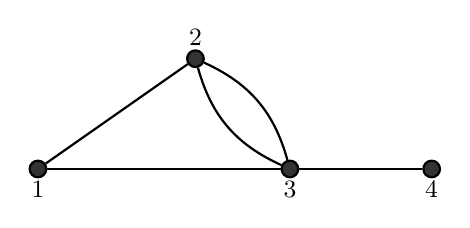
\begin{tikzpicture}[
			every node/.style={circle, draw, fill=black!80, inner sep=0pt, minimum size=6pt},
			lbl/.style={draw=none, fill=none, font=\small},
			thick
			]
			\node[label={[lbl]below:$1$}] (v1) at (0,0) {};
			\node[label={[lbl]above:$2$}] (v2) at (2,1.4) {};
			\node[label={[lbl]below:$3$}] (v3) at (3.2,0) {};
			\node[label={[lbl]below:$4$}] (v4) at (5,0) {};
			\draw (v1) -- (v2);
			\draw (v1) -- (v3);
			\draw[bend left=25]  (v2) to (v3);
			\draw[bend right=25] (v2) to (v3);
			\draw (v3) -- (v4);
		\end{tikzpicture}
	\end{center}
	
	Степени вершин: $d_1=2$, $d_2=3$, $d_3=4$, $d_4=1$. Лапласиан:
	\[
	L_G =
	\begin{pmatrix}
		2 & -1 & -1 &  0 \\
		-1 &  3 & -2 &  0 \\
		-1 & -2 &  4 & -1 \\
		0 &  0 & -1 &  1
	\end{pmatrix}.
	\]
\end{Example}

\subsection{Матричная теорема Кирхгофа}

\begin{Theorem}{Матричная теорема Кирхгофа}{}
	Для любого графа $G$ и любой вершины $i$:
	\[
	\det\!\bigl((L_G)_{ii}\bigr) = \#\{\text{остовных деревьев в } G\},
	\]
	где $(L_G)_{ii}$ — матрица, полученная вычёркиванием $i$-й строки и $i$-го столбца из $L_G$.
\end{Theorem}

\begin{Remark}{}{}
	Для внедиагонального минора также верно:
	$\det\!\bigl((L_G)_{ij}\bigr) = \pm\,\#\{\text{остовных деревьев в } G\}$.
\end{Remark}

\begin{Remark}{}{}
	Если граф $G$ \emph{несвязен} и распадается на две компоненты
	$\{1,\ldots,k\}$ и $\{k{+}1,\ldots,n\}$, то $L_G$ принимает блочно-диагональный вид:
	\[
	L_G =
	\begin{pmatrix}
		L_{G_1} & 0 \\
		0       & L_{G_2}
	\end{pmatrix}.
	\]
	В каждом блоке сумма строк равна нулю, поэтому строки линейно зависимы и
	$\det\!\bigl((L_G)_{ii}\bigr) = 0$ — деревьев нет, что верно.
\end{Remark}

\begin{Example}{Проверка по формуле}{}
	Для графа из предыдущего примера вычислим $\det\!\bigl((L_G)_{11}\bigr)$:
	\[
	\det
	\begin{pmatrix}
		3 & -2 &  0 \\
		-2 &  4 & -1 \\
		0 & -1 &  1
	\end{pmatrix}
	= 12 - 3 - 4 = 5.
	\]
	Граф действительно имеет ровно $5$ остовных деревьев: $1 + 2 + 2 = 5$.
	
	\begin{center}
		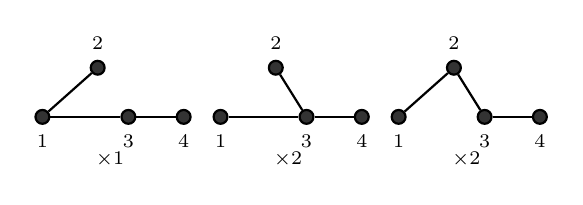
\begin{tikzpicture}[
			scale=0.78,
			v/.style={circle, draw, fill=black!80, inner sep=0pt, minimum size=5pt},
			lbl/.style={font=\scriptsize},
			thick
			]
			% --- дерево 1 (звезда из 3) ---
			\begin{scope}[xshift=0cm]
				\node[v, label={[lbl]below:$1$}] (a1) at (0,0) {};
				\node[v, label={[lbl]above:$2$}] (a2) at (0.9,0.8) {};
				\node[v, label={[lbl]below:$3$}] (a3) at (1.4,0) {};
				\node[v, label={[lbl]below:$4$}] (a4) at (2.3,0) {};
				\draw (a1)--(a2); \draw (a1)--(a3); \draw (a3)--(a4);
				\node[lbl] at (1.1,-0.7) {$\times 1$};
			\end{scope}
			% --- дерево 2a ---
			\begin{scope}[xshift=2.9cm]
				\node[v, label={[lbl]below:$1$}] (b1) at (0,0) {};
				\node[v, label={[lbl]above:$2$}] (b2) at (0.9,0.8) {};
				\node[v, label={[lbl]below:$3$}] (b3) at (1.4,0) {};
				\node[v, label={[lbl]below:$4$}] (b4) at (2.3,0) {};
				\draw (b1)--(b3); \draw (b2)--(b3); \draw (b3)--(b4);
				\node[lbl] at (1.1,-0.7) {$\times 2$};
			\end{scope}
			% --- дерево 3a ---
			\begin{scope}[xshift=5.8cm]
				\node[v, label={[lbl]below:$1$}] (c1) at (0,0) {};
				\node[v, label={[lbl]above:$2$}] (c2) at (0.9,0.8) {};
				\node[v, label={[lbl]below:$3$}] (c3) at (1.4,0) {};
				\node[v, label={[lbl]below:$4$}] (c4) at (2.3,0) {};
				\draw (c1)--(c2); \draw (c2)--(c3); \draw (c3)--(c4);
				\node[lbl] at (1.1,-0.7) {$\times 2$};
			\end{scope}
		\end{tikzpicture}
	\end{center}
\end{Example}

\subsubsection{Доказательство теоремы Кирхгофа}

\begin{proof}
	Доказательство ведётся \textbf{по индукции по числу рёбер} $|E(G)|$.
	
	\medskip
	\textbf{Лемма.} \emph{Если переименовать вершины, ответ не меняется} (первые строки и столбцы переходят в первые при соответствующей перестановке).
	
	\medskip
	\textbf{База: $n = 2$, $k$ кратных рёбер.}
	\[
	L_G =
	\begin{pmatrix} k & -k \\ -k & k \end{pmatrix},
	\qquad
	\det\!\bigl((L_G)_{11}\bigr) = k.
	\]
	Это в точности число остовных деревьев: каждое из $k$ рёбер даёт отдельное дерево.\checkmark
	
	\medskip
	\textbf{Переход.} По лемме можно считать, что ребро $e = \{1,2\}$ существует. Используем
	\emph{тождество удаления-стягивания}:
	\[
	\#\,\text{дер}(G) = \#\,\text{дер}(G{-}e) + \#\,\text{дер}(G{\cdot}e),
	\]
	где $G{-}e$ — граф с удалённым ребром $e$, а $G{\cdot}e$ — граф со стянутым ребром $e$.
	
	Нужно доказать:
	\[
	\det\!\bigl((L_G)_{11}\bigr)
	= \det\!\bigl((L_{G-e})_{11}\bigr) + \det\!\bigl((L_{G\cdot e})_{11}\bigr).
	\]
	
	Матрицы $L_G$ и $L_{G-e}$ отличаются лишь в $2\times2$-блоке на пересечении первых двух строк и столбцов: $d_2$ заменяется на $d_2{-}1$, а $a_{12}=-(\text{кратность } e)$ заменяется на значение без $e$. Разложением по строке, отвечающей вершине $2$, получаем, что ненулевой вклад в разность $\det(L_G)_{11} - \det(L_{G-e})_{11}$ даётся только разностью $(d_2) - (d_2{-}1) = 1$ в диагональной позиции:
	\begin{align*}
		\det\!\bigl((L_G)_{11}\bigr) - \det\!\bigl((L_{G-e})_{11}\bigr)
		&= d_2 \cdot M - (d_2{-}1)\cdot M \\
		&= M = \det\!\bigl((L_{G\cdot e})_{11}\bigr),
	\end{align*}
	где $M$ — соответствующий минор (лапласиан стянутого графа). По индукционному предположению оба слагаемых равны числам деревьев в $G{-}e$ и $G{\cdot}e$.
\end{proof}

\subsection{Деревья в \texorpdfstring{$K_n$}{Kn}. Формула Кэли}

Подсчитаем число остовных деревьев в полном графе $K_n$:

\begin{center}
	\begin{tabular}{c c c}
		\toprule
		$n$ & Число деревьев & $n^{n-2}$ \\
		\midrule
		$1$ & $1$ & $1^{-1} = 1$ \\
		$2$ & $1$ & $2^{0} = 1$ \\
		$3$ & $3$ & $3^{1} = 3$ \\
		$4$ & $16$ & $4^{2} = 16$ \\
		$5$ & $125$ & $5^{3} = 125$ \\
		\bottomrule
	\end{tabular}
\end{center}

Закономерность: число деревьев в $K_n$ равно $n^{n-2}$.

\begin{Remark}{}{}
	Для $n=4$ все $16$ остовных деревьев распадаются на два вида:
	$4$ звезды (одна центральная вершина степени~$3$) и $12$ путей ($4!/2 = 12$).
	Для $n=5$ три вида: $5$ звёзд, $60$ путей ($5!/2$) и ещё $60$ деревьев с развилкой, итого $5 + 60 + 60 = 125$.
	
	\begin{center}
		\begin{tikzpicture}[
			v/.style={circle, draw, fill=black!80, inner sep=0pt, minimum size=5pt},
			lbl/.style={font=\scriptsize}, thick, scale=0.85
			]
			% K_3
			\begin{scope}[xshift=0cm, yshift=0cm]
				\node[v] (t1) at (0,0.7) {};
				\node[v] (t2) at (-0.6,0) {};
				\node[v] (t3) at (0.6,0) {};
				\draw (t1)--(t2); \draw (t1)--(t3); \draw (t2)--(t3);
				\node[lbl] at (0,-0.5) {$K_3$, три дерева};
			\end{scope}
			% K_4
			\begin{scope}[xshift=4cm, yshift=0cm]
				\node[v] (q1) at (0,0.8) {};
				\node[v] (q2) at (-0.8,0) {};
				\node[v] (q3) at (0,0) {};
				\node[v] (q4) at (0.8,0) {};
				\draw (q1)--(q2); \draw (q1)--(q3); \draw (q1)--(q4);
				\draw (q2)--(q3); \draw (q2)--(q4); \draw (q3)--(q4);
				\node[lbl] at (0,-0.5) {$K_4$, 16 деревьев};
			\end{scope}
		\end{tikzpicture}
	\end{center}
\end{Remark}

\begin{Theorem}{Формула Кэли}{}
	В полном графе $K_n$ ровно $n^{n-2}$ остовных деревьев.
\end{Theorem}

\begin{proof}
	По теореме Кирхгофа достаточно вычислить $\det\!\bigl((L_{K_n})_{11}\bigr)$.
	
	Лапласиан $K_n$ имеет вид: на диагонали стоят $n{-}1$, вне диагонали $-1$. Минор
	$(L_{K_n})_{11}$ — матрица $(n{-}1)\times(n{-}1)$:
	\[
	M = \begin{pmatrix}
		n{-}1 & -1 & \cdots & -1 \\
		-1 & n{-}1 & \cdots & -1 \\
		\vdots & & \ddots & \vdots \\
		-1 & -1 & \cdots & n{-}1
	\end{pmatrix}.
	\]
	
	\textbf{Шаг 1.} Вычтем строку~$1$ из каждой строки $2, \ldots, n{-}1$. Строка $k$ ($k \ge 2$) принимает вид $(\underbrace{-n}_{1}, \underbrace{0, \ldots, n, \ldots, 0}_{k\text{-я поз.}})$:
	\[
	\det M = \det
	\begin{pmatrix}
		n{-}1 & -1 & \cdots & -1 \\
		-n & n & & 0 \\
		\vdots & & \ddots & \\
		-n & 0 & & n
	\end{pmatrix}.
	\]
	
	\textbf{Шаг 2.} Выносим $n$ из каждой из строк $2, \ldots, n{-}1$ (всего $n{-}2$ строки):
	\[
	\det M = n^{n-2} \cdot \det
	\begin{pmatrix}
		n{-}1 & -1 & \cdots & -1 \\
		-1 & 1 & & 0 \\
		\vdots & & \ddots & \\
		-1 & 0 & & 1
	\end{pmatrix}.
	\]
	
	\textbf{Шаг 3.} Прибавим ко строке~$1$ все строки $2, \ldots, n{-}1$. Первая строка превращается в $(1, 0, \ldots, 0)$, и определитель нижнетреугольной матрицы равен~$1$:
	\[
	\det M = n^{n-2} \cdot \det
	\begin{pmatrix}
		1 & 0 & \cdots & 0 \\
		-1 & 1 & & 0 \\
		\vdots & & \ddots & \\
		-1 & 0 & & 1
	\end{pmatrix}
	= n^{n-2} \cdot 1 = n^{n-2}. 
	\]
\end{proof}

\subsection{Взвешенные ориентированные ациклические графы}


\begin{Definition}{Взвешенный орграф}{}
	\emph{Взвешенный ориентированный ациклический граф} (dag) — ориентированный граф $G$ без ориентированных циклов, в котором каждому ребру $e$ сопоставлено вещественное число $w(e)$ (\emph{вес ребра}).
\end{Definition}

\begin{Definition}{Вес пути и весовая функция}{}
	Для ориентированного пути $P = e_1, e_2, \ldots, e_k$ его \emph{вес}:
	\[
	w(P) = w(e_1)\cdot w(e_2) \cdots w(e_k).
	\]
	Для вершин $a, b \in V(G)$ определяем:
	\[
	w(a,b) = \sum_{P:\,a \to b} w(P),
	\]
	где суммирование ведётся по всем ориентированным путям из $a$ в $b$.
\end{Definition}

\begin{Remark}{}{}
	Если ребро $e$ с весом $w$ заменить двумя параллельными рёбрами с весами $w_1$ и $w_2$,
	где $w_1 + w_2 = w$, то $w(a,b)$ для всех пар $(a,b)$ не изменится.
\end{Remark}

\begin{Example}{Пример взвешенного орграфа}{}
	Рассмотрим двудольный орграф с вершинами $\{1,2,3\}$ (источники) и $\{4,5,6\}$ (стоки),
	в котором из каждого источника идут пути ко всем стокам через промежуточные вершины,
	все веса рёбер $w_i = 1$.
	
	\begin{center}
		\begin{tikzpicture}[
			->, >=Stealth,
			v/.style={circle, draw, fill=black!80, inner sep=0pt, minimum size=6pt},
			m/.style={circle, draw, fill=black!20, inner sep=1pt, minimum size=16pt},
			lbl/.style={font=\small},
			thick
			]
			\node[v, label={[lbl]left:$1$}] (s1) at (0,3) {};
			\node[v, label={[lbl]left:$2$}] (s2) at (0,2) {};
			\node[v, label={[lbl]left:$3$}] (s3) at (0,1) {};
			
			\node[m] (x1) at (2,3.5) {$x_1$};
			\node[m] (x2) at (2,2.5) {$x_2$};
			\node[m] (x3) at (2,1.5) {$x_3$};
			\node[m] (x4) at (2,0.5) {$x_4$};
			
			\node[v, label={[lbl]right:$4$}] (t1) at (4,3) {};
			\node[v, label={[lbl]right:$5$}] (t2) at (4,2) {};
			\node[v, label={[lbl]right:$6$}] (t3) at (4,1) {};
			
			% sources to intermediate vertices
			\draw (s1) -- (x1);
			\draw (s1) -- (x2);
			
			\draw (s2) -- (x1);
			\draw (s2) -- (x2);
			\draw (s2) -- (x3);
			
			\draw (s3) -- (x1);
			\draw (s3) -- (x2);
			\draw (s3) -- (x3);
			\draw (s3) -- (x4);
			
			% intermediate vertices to sinks
			\draw (x1) -- (t1);
			\draw (x1) -- (t2);
			\draw (x1) -- (t3);
			
			\draw (x2) -- (t2);
			\draw (x2) -- (t3);
			
			\draw (x3) -- (t2);
			\draw (x3) -- (t3);
			
			\draw (x4) -- (t3);
		\end{tikzpicture}
	\end{center}
	
	Подсчитанные весовые суммы путей:
	\[
	\bigl(w(a_i, b_j)\bigr) =
	\begin{pmatrix}
		w(1,4) & w(1,5) & w(1,6) \\
		w(2,4) & w(2,5) & w(2,6) \\
		w(3,4) & w(3,5) & w(3,6)
	\end{pmatrix}
	=
	\begin{pmatrix}
		1 & 2 & 2 \\
		1 & 3 & 3 \\
		1 & 3 & 4
	\end{pmatrix}.
	\]
	Определитель:
	\[
	\det
	\begin{pmatrix}
		1 & 2 & 2 \\
		1 & 3 & 3 \\
		1 & 3 & 4
	\end{pmatrix}
	= 1\cdot(12-9) - 2\cdot(4-3) + 2\cdot(3-3) = 3 - 2 + 0 = 1.
	\]
\end{Example}


\subsection{Теорема Бесселя--Линдстрёма--Гесселя--Вьенно (БЛГВ)}

\begin{Theorem}{Теорема БЛГВ}{}
	Пусть $G$ — взвешенный ориентированный ациклический граф,
	$A = \{a_1, \ldots, a_n\}$ и $B = \{b_1, \ldots, b_n\}$ — два набора вершин. Тогда:
	\[
	\det\!\bigl(w(a_i, b_j)\bigr)_{1\le i,j\le n}
	=
	\sum_{\substack{(P_1,\ldots,P_n) \\ \text{не пересекаются}}}
	w(P_1)\cdots w(P_n)\cdot\operatorname{sign}(P_1,\ldots,P_n),
	\]
	где суммирование ведётся по системам попарно \emph{непересекающихся} путей
	$P_i : a_i \to b_{\pi(i)}$
	($\pi$ — некоторая перестановка), а
	$\operatorname{sign}(P_1,\ldots,P_n) = \operatorname{sign}(\pi)$.
\end{Theorem}

\begin{proof}
	\textbf{Шаг 1. Раскрытие определителя.}
	
	По определению:
	\begin{align*}
		\det\!\bigl(w(a_i,b_j)\bigr)
		&= \sum_{\pi\in S_n} \operatorname{sign}(\pi)\cdot
		w(a_1, b_{\pi(1)}) \cdots w(a_n, b_{\pi(n)}) \\
		&= \sum_{\pi} \operatorname{sign}(\pi)
		\!\!\!\!\sum_{\substack{P_1:\,a_1 \to b_{\pi(1)}}}\!\!\! w(P_1)
		\;\cdots\!\!\!\!
		\sum_{\substack{P_n:\,a_n \to b_{\pi(n)}}}\!\!\! w(P_n) \\
		&= \sum_{\substack{(P_1,\ldots,P_n) \\ P_i:\,a_i \to b_{\pi(i)}}}
		w(P_1)\cdots w(P_n)\cdot\operatorname{sign}(P_1,\ldots,P_n).
	\end{align*}
	
	\textbf{Шаг 2. Обнуление пересекающихся систем.}
	
	Разобьём сумму на две части:
	\[
	\underbrace{\sum_{\text{не пересекаются}}}_{=\,\text{правая часть теоремы}}
	+
	\underbrace{\sum_{\text{есть пересечение}}}_{=\,?}.
	\]
	Достаточно показать, что вторая сумма равна нулю. Определим \textbf{инволюцию}
	$\operatorname{inv}$ на пересекающихся системах следующим образом.
	
	Пусть $(P_1,\ldots,P_n)$ — система с хотя бы одним пересечением. Определим:
	\begin{enumerate}
		\item $t = \min\{i : P_i \text{ пересекает } P_j \text{ для некоторого } j>i\}$,
		\item $x$ — \emph{первая} вершина на $P_t$, принадлежащая какому-либо $P_s$, $s > t$,
		\item $s = \min\{j > t : x \in P_j\}$.
	\end{enumerate}
	
	\begin{center}
		\begin{tikzpicture}[
			->, >=Stealth,
			v/.style={circle, draw, fill=black!80, inner sep=0pt, minimum size=5pt},
			lbl/.style={font=\small},
			thick
			]
			% Путь P_t: a_t -> x -> конец
			\draw[blue, thick] (0,1) -- node[above, lbl, black]{$P_t$} (2,1) 
			-- (3,0) -- node[below, lbl, black]{} (5,0.3);
			% Путь P_s: a_s -> x -> конец
			\draw[red!70!black, thick] (0,0) -- node[below, lbl, black]{$P_s$} (3,0) 
			-- (5,1.3);
			% точка пересечения
			\node[v, fill=orange] (x) at (3,0) {};
			\node[lbl] at (3,-0.35) {$x$};
			% метки источников
			\node[v] at (0,1) {};
			\node[v] at (0,0) {};
			\node[lbl] at (-0.35,1) {$a_t$};
			\node[lbl] at (-0.35,0) {$a_s$};
			% метки стоков
			\node[lbl] at (5.3,0.3) {$b_{\pi(t)}$};
			\node[lbl] at (5.3,1.3) {$b_{\pi(s)}$};
			% стрелки-намёки на inv
			\draw[blue, thick, dashed] (3,0) -- (5,1.3);
			\draw[red!70!black, thick, dashed] (3,0) -- (5,0.3);
		\end{tikzpicture}
	\end{center}
	
	Положим $\operatorname{inv}(P_1,\ldots,P_n) = (P_1,\ldots,P_t',\ldots,P_s',\ldots,P_n)$, где:
	\begin{itemize}
		\item $P_t'$: из $a_t$ до $x$ вдоль $P_t$, затем из $x$ до конца вдоль $P_s$\,,
		\item $P_s'$: из $a_s$ до $x$ вдоль $P_s$, затем из $x$ до конца вдоль $P_t$\,.
	\end{itemize}
	Это \emph{транспозиция хвостов} путей $P_t$ и $P_s$ после точки $x$.
	
	\medskip
	\textbf{Утверждение 1: $\operatorname{inv}\circ\operatorname{inv} = \mathrm{id}$.}
	Действительно, для новой системы $(P_1,\ldots,P_t',\ldots,P_s',\ldots,P_n)$:
	\begin{itemize}
		\item $P_1,\ldots,P_{t-1}$ по-прежнему ни с кем не пересекаются (они не изменились),
		\item $P_t'$ пересекает $P_s'$ в точке $x$, причём $x$ — первая точка пересечения и $t' = t$, $s' = s$,
		\item $P_{t+1},\ldots,P_{s-1}$ не пересекали $P_t$ до $x$ $\Rightarrow$ не пересекают $P_t'$ до $x$.
	\end{itemize}
	Применив $\operatorname{inv}$ повторно, получим исходную систему.
	
	\medskip
	\textbf{Утверждение 2: знак меняется.}
	При переходе к $\operatorname{inv}$ конечные вершины путей $P_t$ и $P_s$ меняются местами
	($b_{\pi(t)} \leftrightarrow b_{\pi(s)}$), что отвечает транспозиции в перестановке $\pi$:
	\[
	\operatorname{sign}\!\bigl(\operatorname{inv}(P_1,\ldots,P_n)\bigr) = -\operatorname{sign}(P_1,\ldots,P_n).
	\]
	
	Таким образом, $\operatorname{inv}$ разбивает пересекающиеся системы на пары с противоположными
	знаками и одинаковым произведением весов. Вклады в сумму попарно сокращаются:
	\[
	\sum_{\text{есть пересечение}}
	w(P_1)\cdots w(P_n)\cdot\operatorname{sign}(P_1,\ldots,P_n) = \sum\nolimits_{\text{пары}} 0 = 0.
	\]
	Теорема доказана.
\end{proof}